\documentclass[../main/report.tex]{subfiles}
\begin{document}

\subsection{HDMI}
\begin{figure}
	\centering
	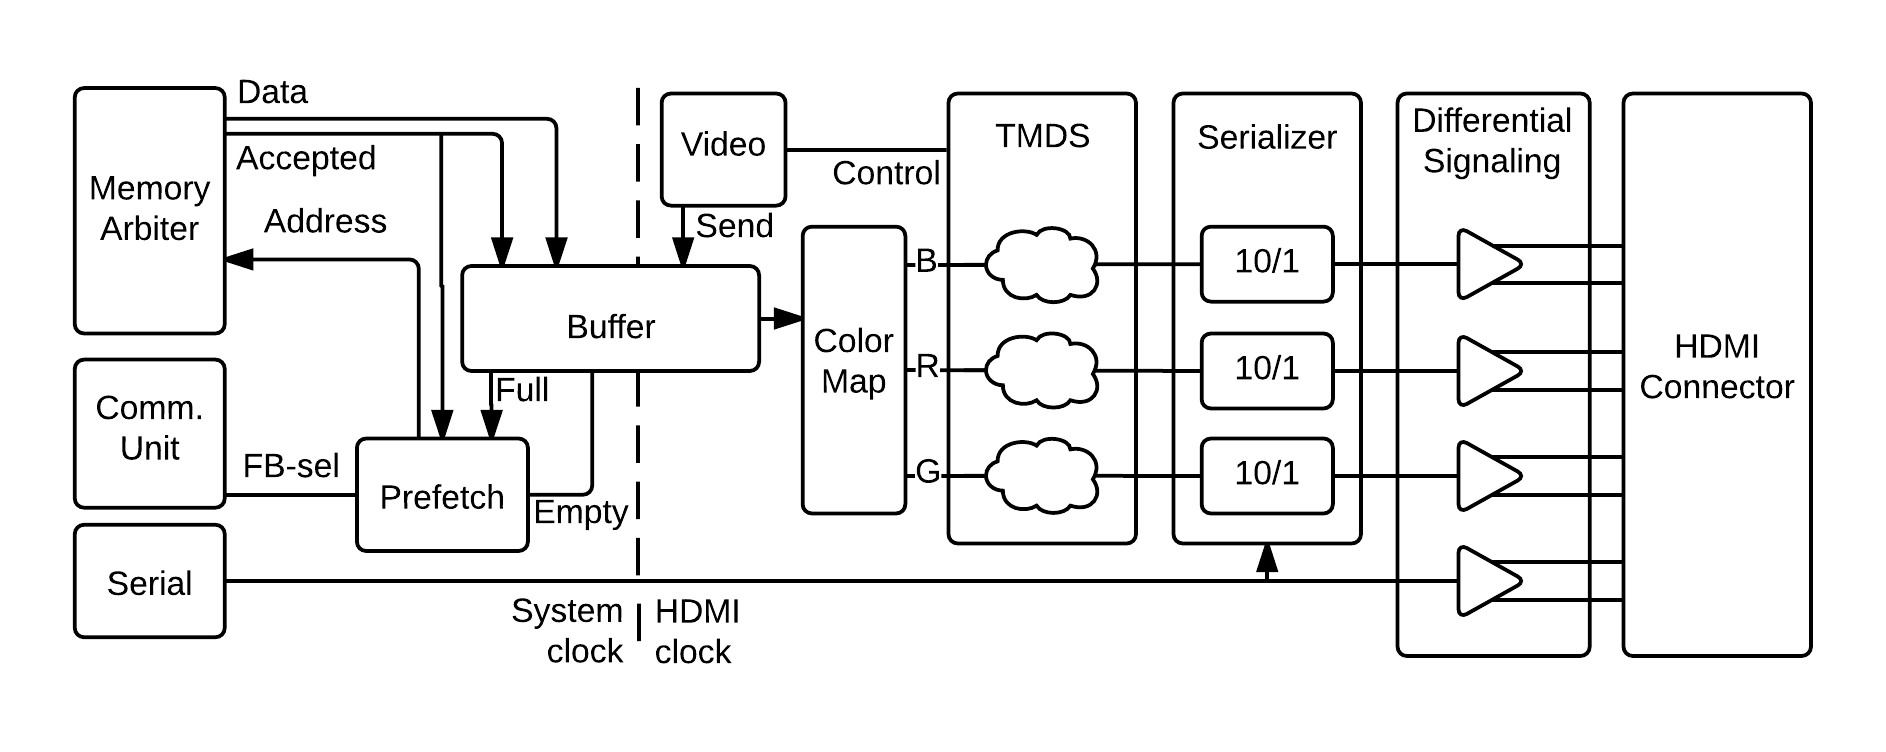
\includegraphics[width=\textwidth]{diagrams/HDMI_overview.png}
	\caption{
		The logical overview of the video unit.
		A prefetching unit tries to fill the buffer when it is not full.
		The \emph{Accepted} signal signifies a sucessful memory request.
		Across the clock domain boundary, the video timing unit generates control signals.
		When pixel data should be transferred, the \emph{Send} signal moves pixels from the buffer to the transmission units.
		The 16-bit pixel data is converted to three 8-bit colors, TMDS encoded, serialized and output using differential signaling.
		Should the buffer go empty, the prefetch unit needs to immediately advance to the next pixel to stay synchronized with the timing unit.
	}
	\label{fig:video_unit}
\end{figure}
From a demo makers perspective, a GPU without a video output is commonly known as a space heater.
Demolicious uses HDMI for its video output, making it easy to connect to any recent video display.

HDMI is a streaming protocol; the receiver reads data from the cable at a fixed rate.
In Demolicious, the GPU has priority access to the memory.
This means that the video unit may not have access to the framebuffer (which lies in memory) when it's time to send a pixel.
To alleviate this issue, as much of the framebuffer as possible is prefetched into a buffer whenever memory is idle.
Should the buffer underflow, sending of late pixels must be abandoned.
Otherwise, pixels will not be synchronized with the position they should appear at on the screen.

Control signals assert where in the data stream a new frame of video starts and ends.
These allow the receiver to determine the resolution and refresh rate of the video.

The lowest resolution supported by HDMI is 640x480.
As this is larger than our framebuffers (64 x 64 pixels), a letterbox is added around the picture.
For debugging purposes, the letterbox consists of a low-contrast checker pattern.

To actually send the data over HDMI, control signals and pixel data are split into three channels.
They are then encoded using a scheme known as TMDS.
The purpose of TMDS is to minimize the effect of noise over the physical connection.

TMDS uses 10 bits to encode either an 8-bit color value when sending a image, or control values when not.
Demolicious uses a 16-bit word size, so colors are represented with 5 bits for red, 6 for green and 5 for blue.
These are resized to 8-bit values using a scheme that allows for both complete black and white colors.
Each channel is then serialized before being output together with a clock using differential-signaling.

Finally, to avoid a visual artifact known as \emph{screen tearing}, a technique known as \emph{V-sync} with \emph{double buffering} is used.
These techniques ensure that only complete frames of video are output, increasing visual fidelity.

\end{document}
